\newpage
\section{Question 8}
	\subsection{}
	For complete working out see the Appendix.
	\newline Brief overview of methodology:\newline
	By differentiating the position of link 2 we obtain its velocity. From there we can determine the systems Kinetic Energy.\newline
	Potential Energy can be found straight from the effect of gravity.\newline
	From there, we can find the Lagrangian $L = K - P$.\newline
	We can then determine $T1$ and $T2$ from the Lagrangian.\newline
	\newline
	Final Results:\newline
	After substituting in for $m_{i}$, $l_{i}$, $I_{i}$, we obtain the following:\newline \newline
	\hspace{20mm}$T_{1} = \alpha _{1} [5.1625 + 3\cos \theta _{2}] + \alpha _{2} [0.7625 + 1.5\cos \theta _{2}]$\newline
	\hspace{30mm}$ - \omega _{1} \omega _{2} [3\sin \theta _{2}] - \omega ^2 _{2}[3\sin \theta _{2}] $\newline
	\hspace{40mm}$ + 6.5g\cos \theta _{1} + 1.5g\cos (\theta _{1} + \theta _{2})$\newline\newline
	and\newline\newline
	\hspace{20mm}$T_{2} = \alpha _{1} [0.7625 + 1.5\cos \theta _{2}] + \alpha _{2} [0.2]$\newline
	\hspace{30mm}$ + \omega ^2 _{1}[1.5\sin \theta _{2}] + 1.5g\cos (\theta _{1} + \theta _{2})$\newline\newline
	where\newline\newline
		$g = 9.81$ is the acceleration due to gravity.\newline
		$\omega _{i} = \frac{d}{dt} \theta _{i}$ is the angular velocity.\newline
		$\alpha _{i} = \frac{d}{dt} \omega _{i}$ is the angular acceleration.\newline
	\pagebreak	
	\subsection{}
	Rearranging the above equations so that $\alpha _{i}$ is the subject we obtain the following:\newline\newline
	$ \alpha _{1} = \frac{T_{1} - \alpha _{2}[0.7625 + 1.5\cos \theta _{2}] + \omega _{1}\omega _{2}[3\sin \theta _{2}] + \omega^2 _{2}[3\sin \theta _{2}] - 6.5g\cos (\theta _{1} + \theta _{2})}{5.1625 + 3\cos \theta _{2}} $\newline 
	\hspace{20mm}$==> Equation 1$\newline\newline
	$ \alpha _{2} = \frac{T_{2} - \alpha _{1}[0.7625 + 1.5\cos \theta _{2}] - \omega^2 _{1}[1.5\sin \theta _{2}] - 1.5g\cos (\theta _{1} + \theta _{2})}{0.2} $\newline 
	\hspace{20mm}$==> Equation 2$\newline\newline
	\newline
	Through matlab we can simultaneously solve $Equations$ $1$ and $2$ to obtain a description of $\alpha _{i}$ without depending on the other $\alpha _{i}$.\newline
	See the Appendix for Question 8 for the matlab code.\newline
%		insert matlab script here
%see appendix?
	This enables us to utilise the following simulink model:\newline
%insert simulink image
	\begin{figure}[position = here]
		\begin{centering}
			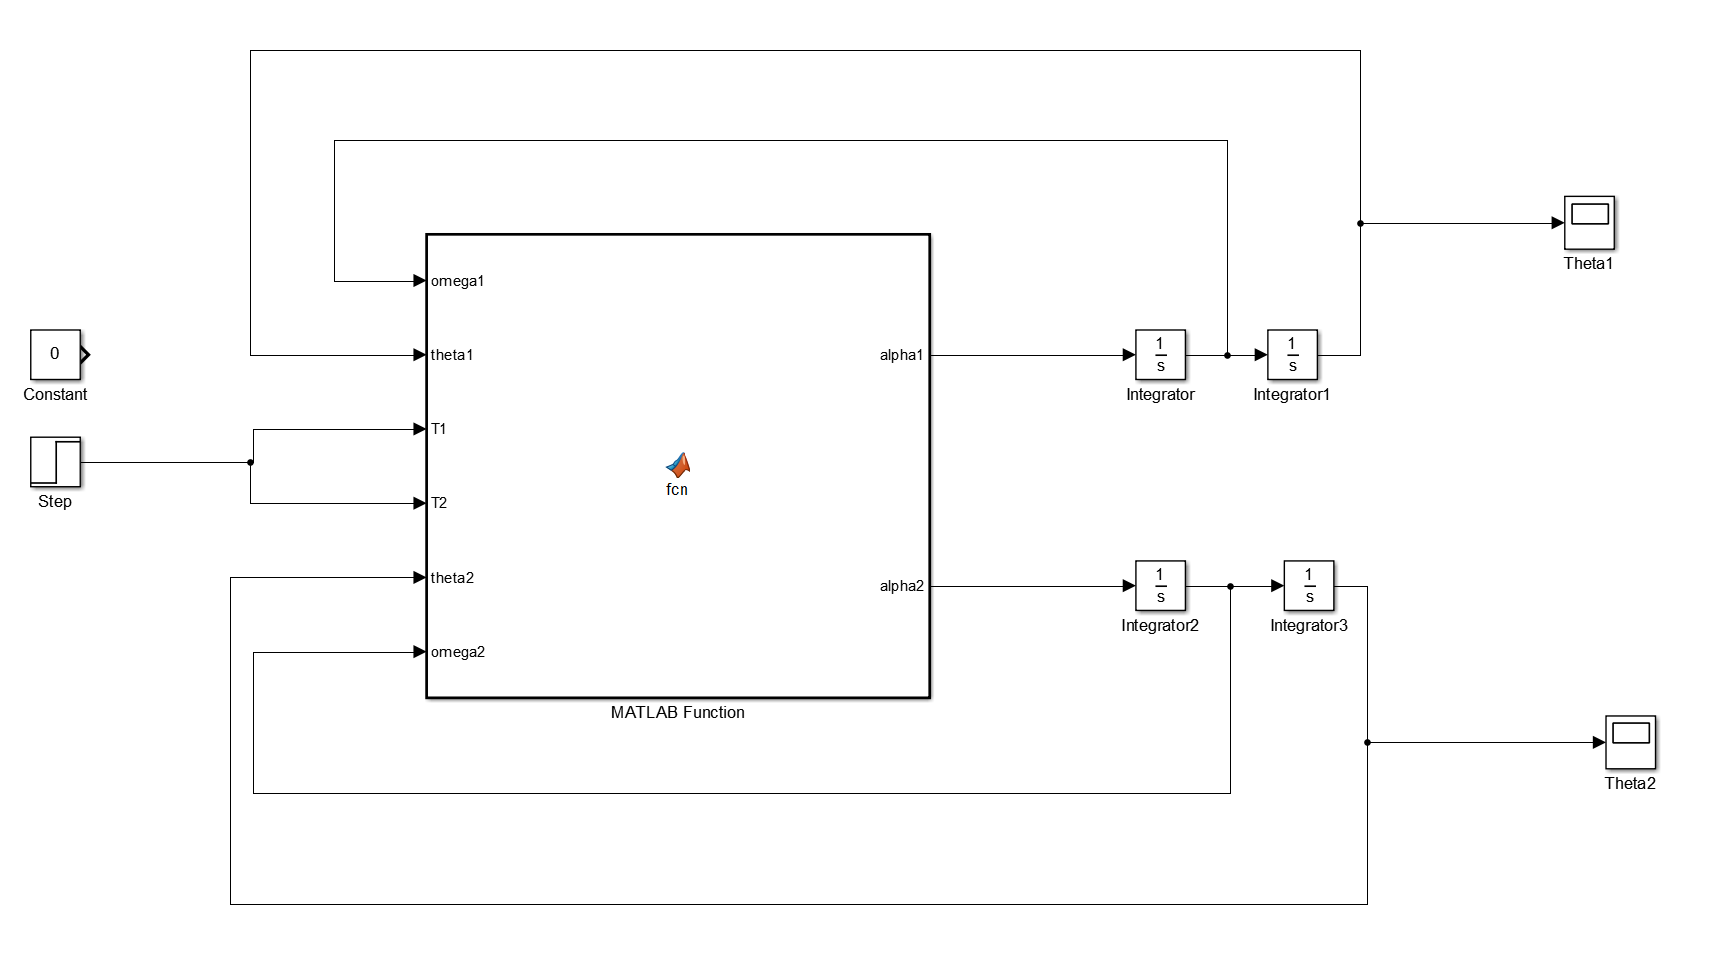
\includegraphics[scale=0.5]{q8_simulink}\\
			\caption [WSpace]{Simulink Model}
		\end{centering}
	\end{figure}
	\newline
	\pagebreak
	For a constant zero input torque, we obtain for $\theta _{1}$ the following output:\newline
	%insert Theta1_constant_zero.jpg
	\begin{figure}[position = here]
		\begin{centering}
			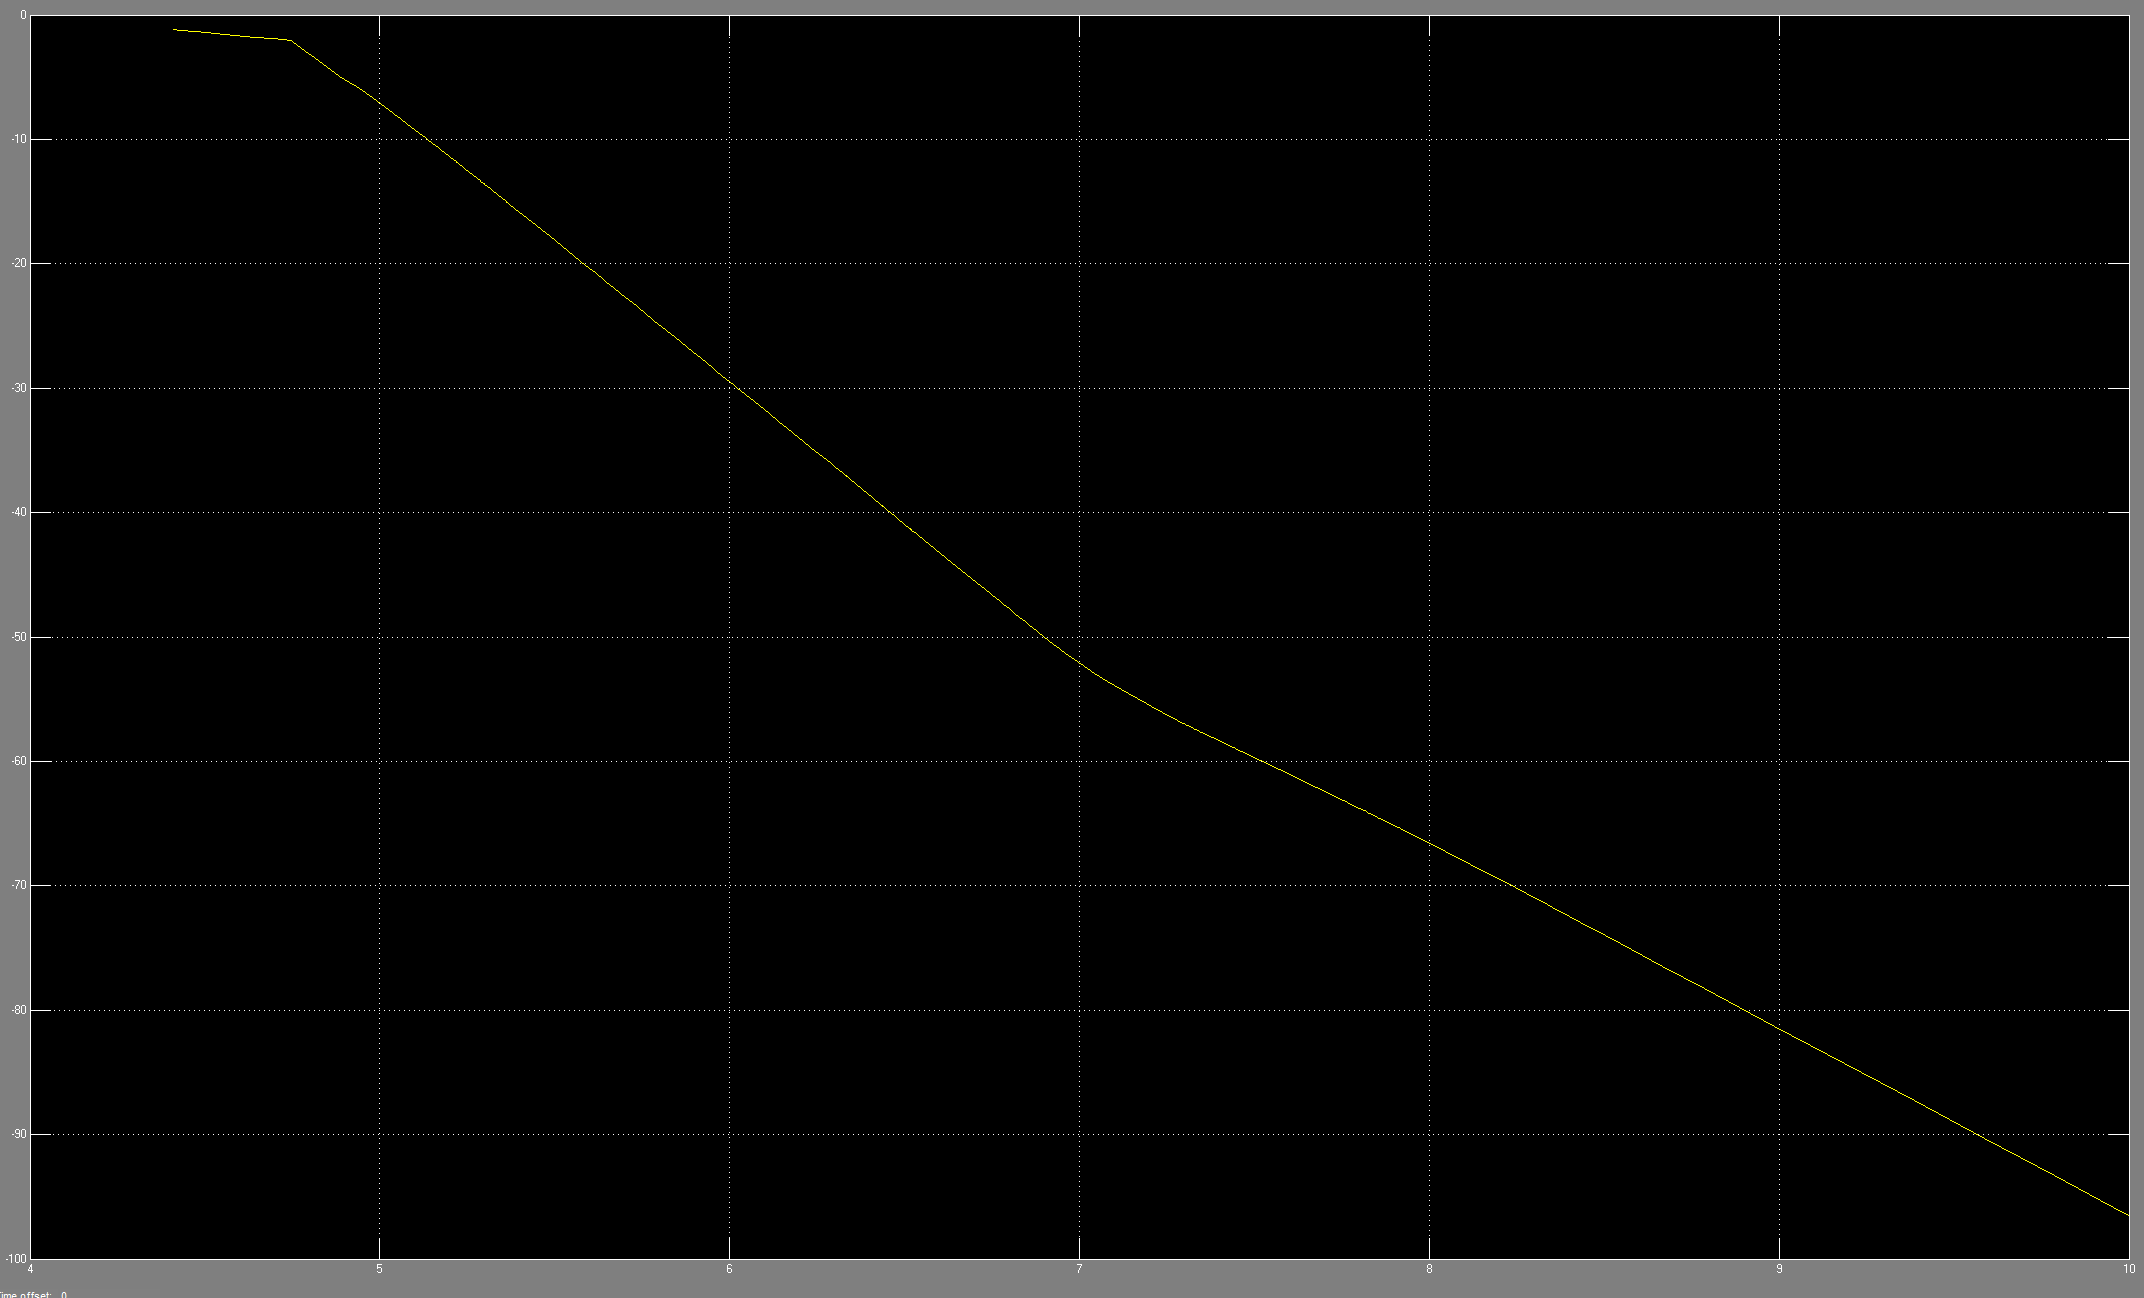
\includegraphics[scale=0.3]{q8_Theta1_constant_zero}\\
			\caption [WSpace]{Theta 1 for constant zero torque}
		\end{centering}
	\end{figure}
	
	\newline and for $\theta _{2}$:\newline
	%insert Theta2_constant_zero.jpg
	\begin{figure}[position = here]
		\begin{centering}
			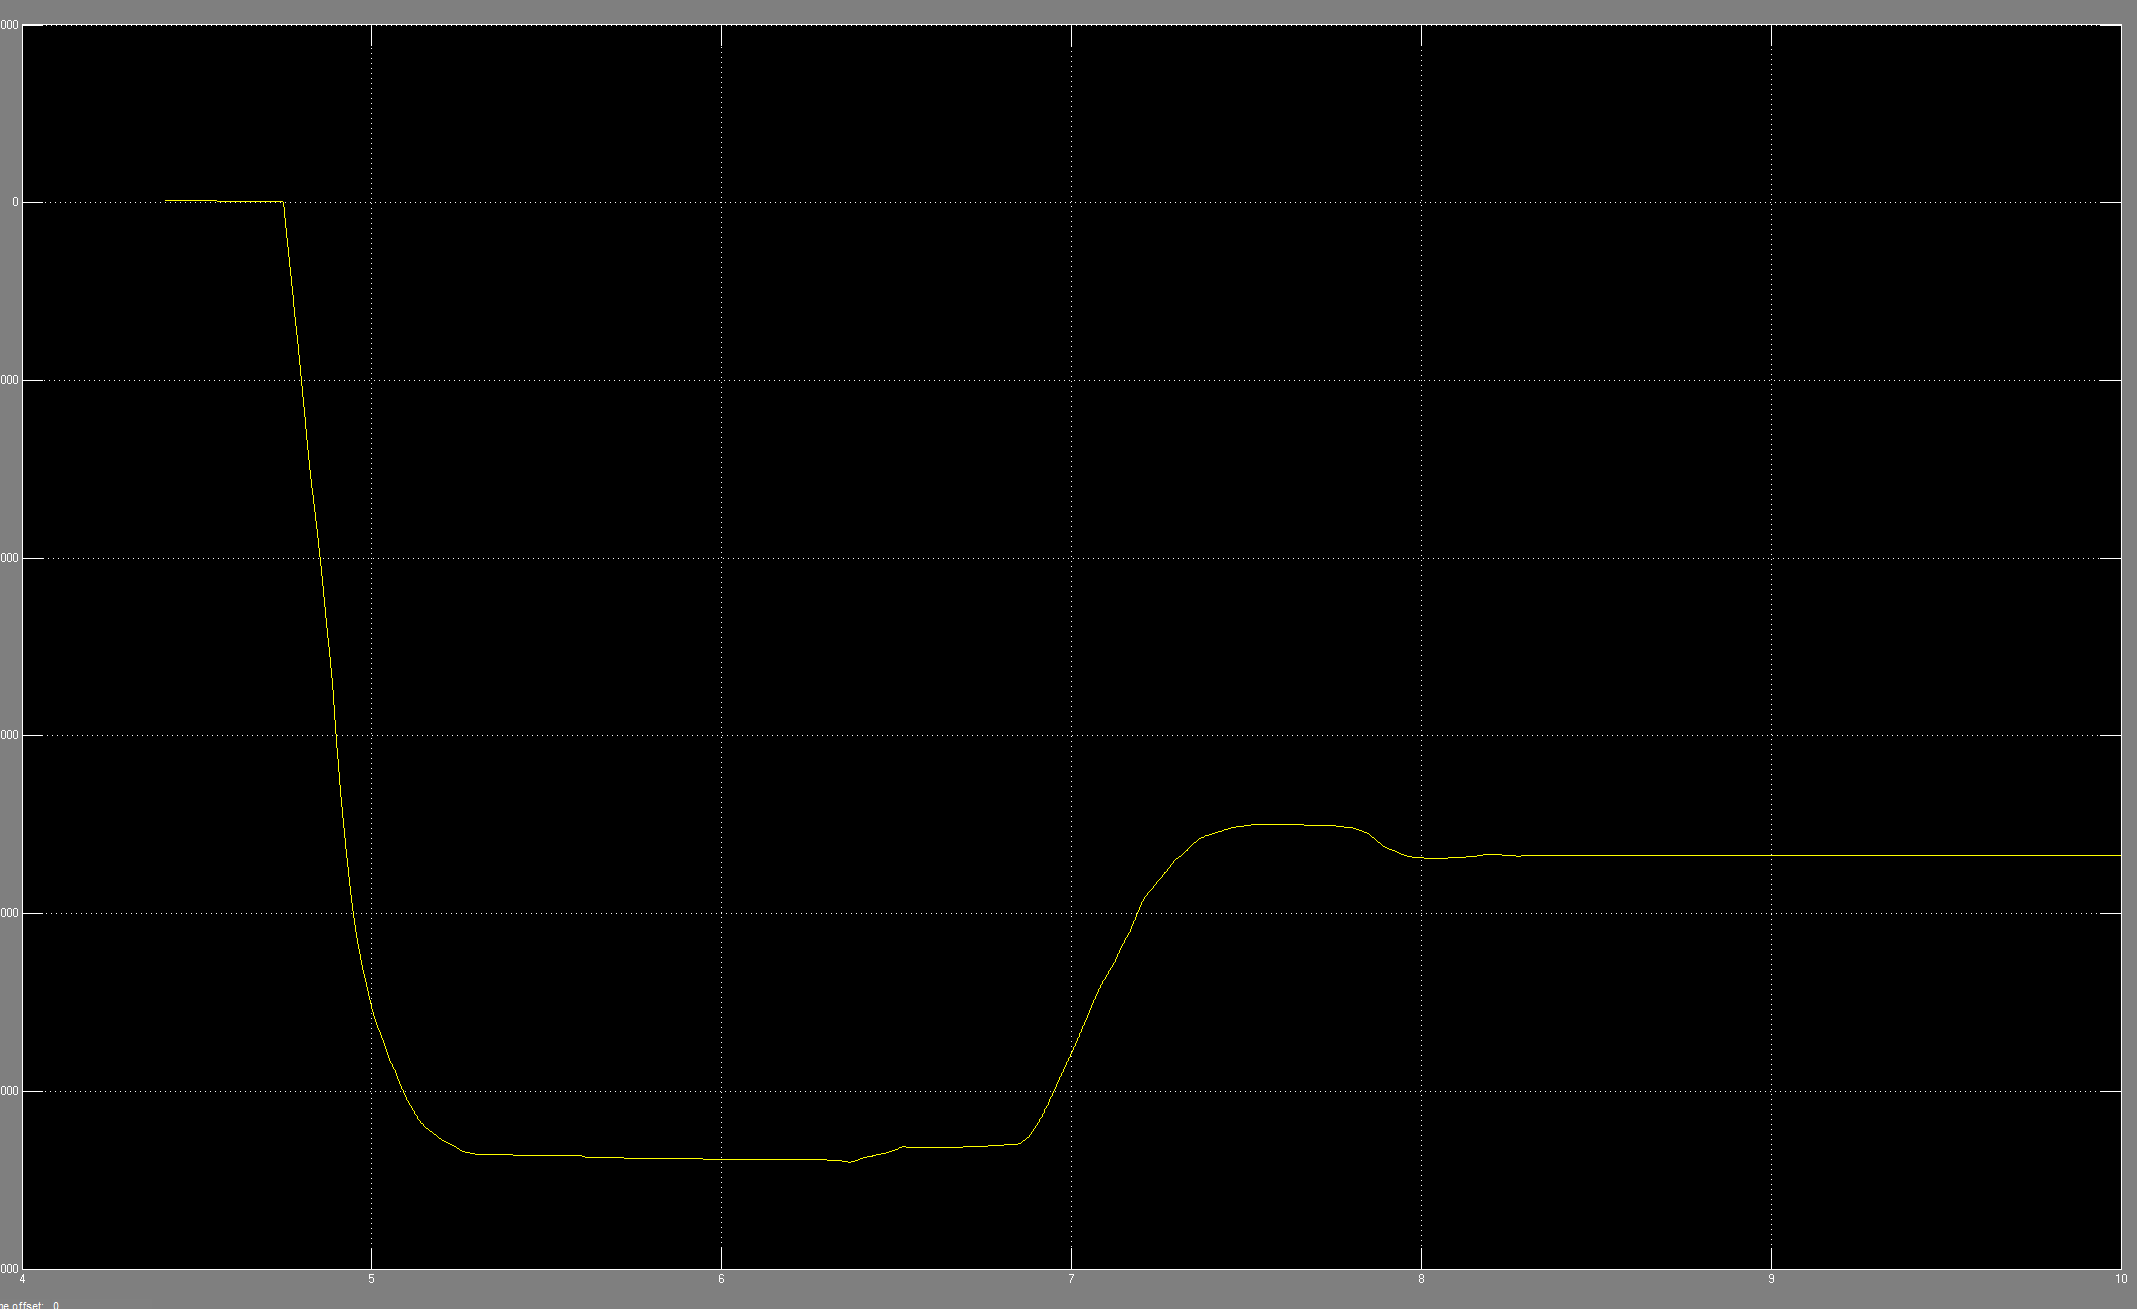
\includegraphics[scale=0.3]{q8_Theta2_constant_zero}\\
			\caption [WSpace]{Theta 2 for constant zero torque}
		\end{centering}
	\end{figure}
	\pagebreak
	\newline For a step input torque, we obtain for $\theta _{1}$:\newline
	%insert Theta1_step.jpg
	\begin{figure}[position = here]
		\begin{centering}
			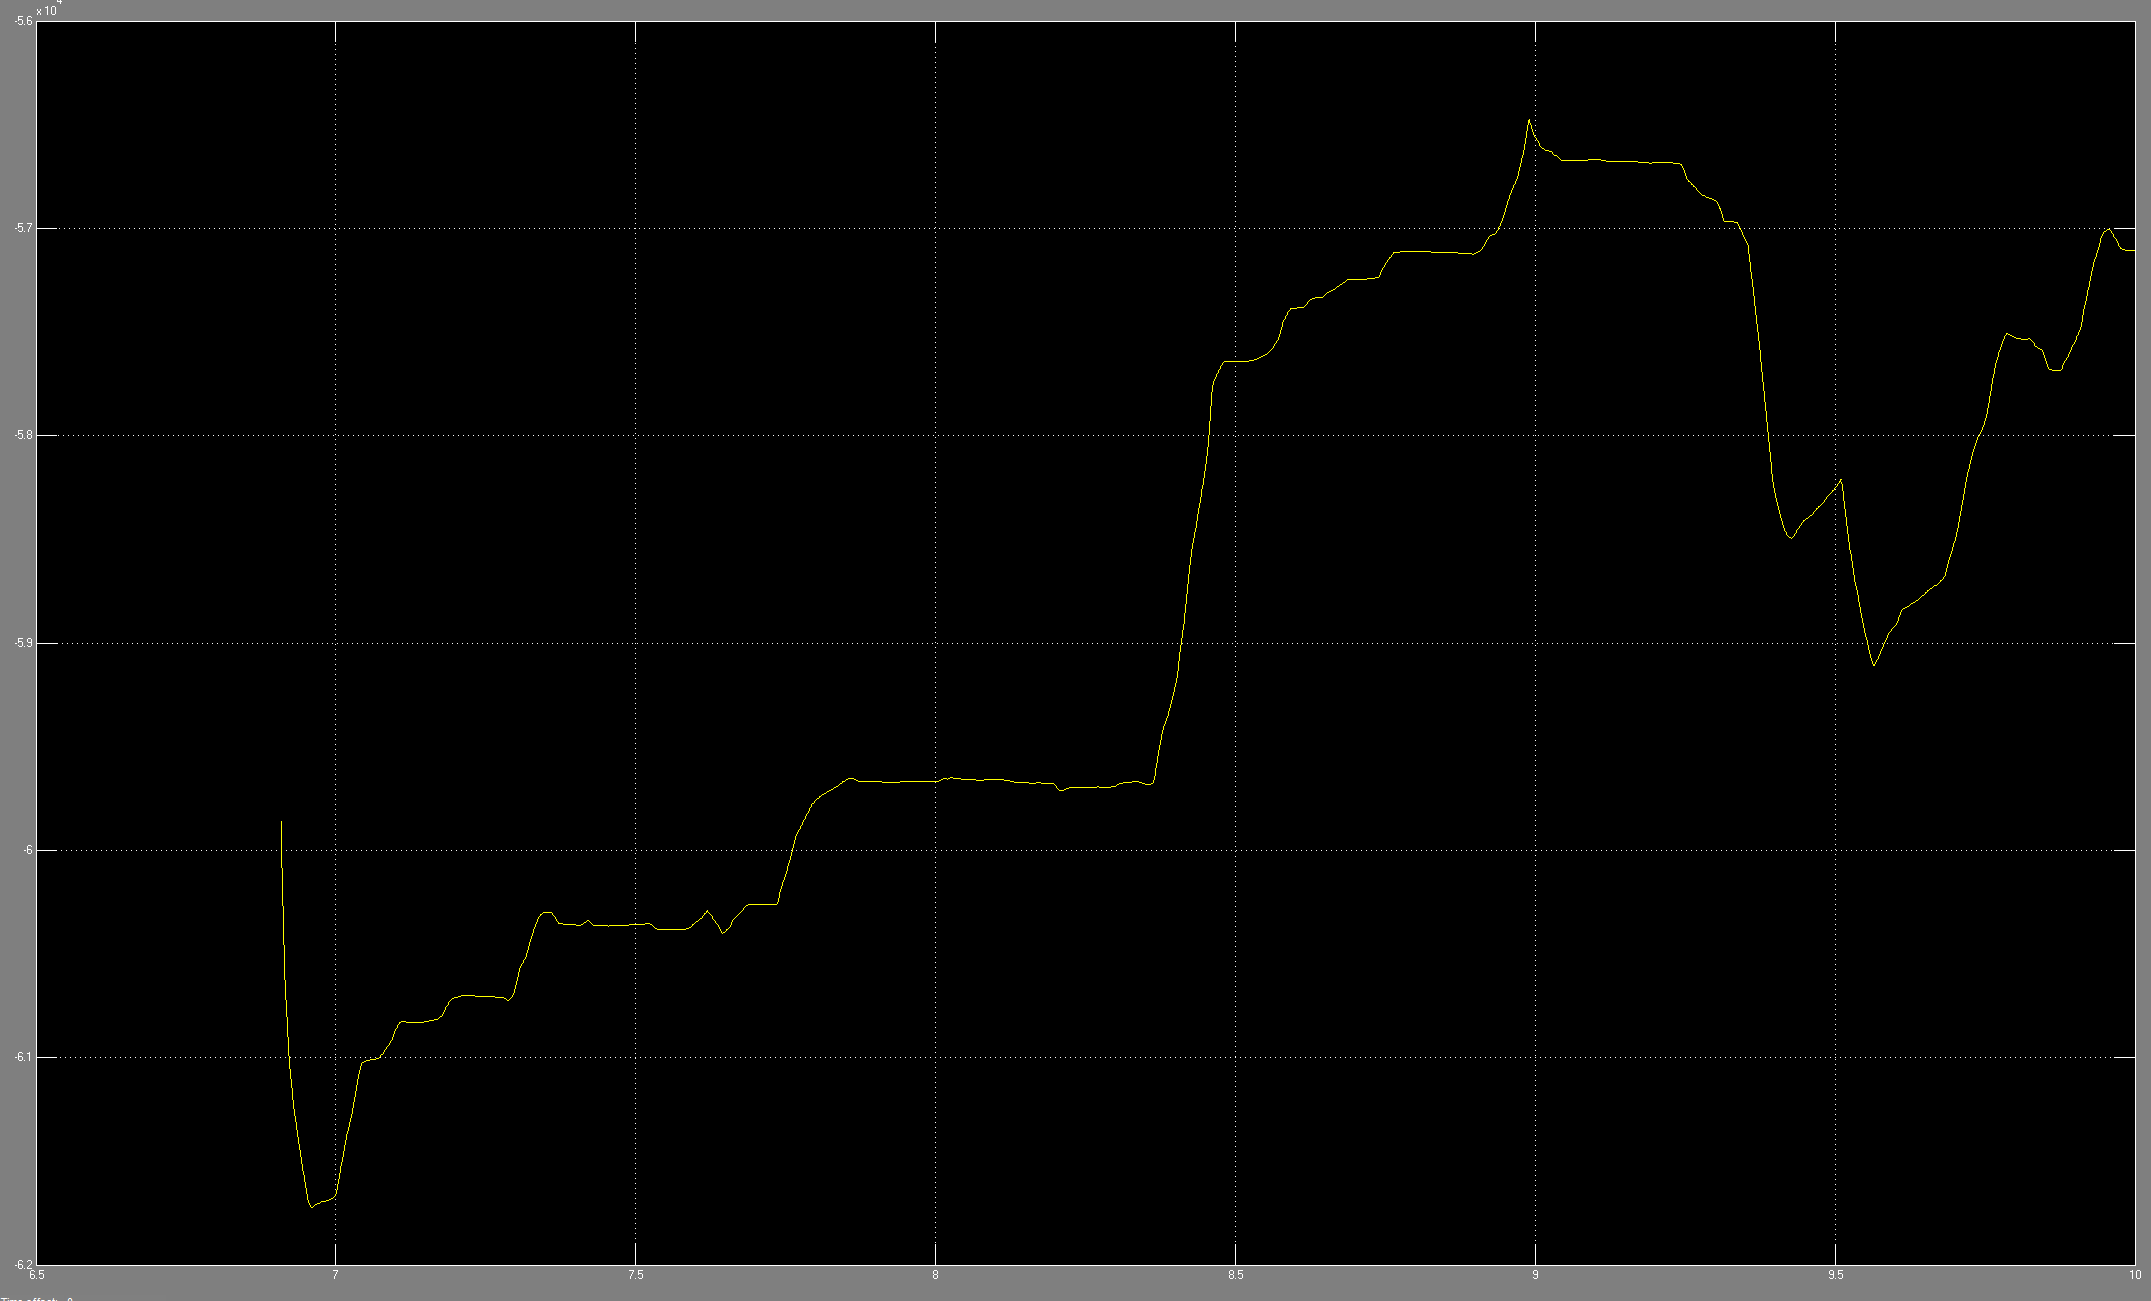
\includegraphics[scale=0.3]{q8_Theta1_step}\\
			\caption [WSpace]{Theta 1 for step torque}
		\end{centering}
	\end{figure}
	\newline and for $\theta _{2}$:\newline
	%insert Theta2_step.jpg
	\begin{figure}[position = here]
		\begin{centering}
			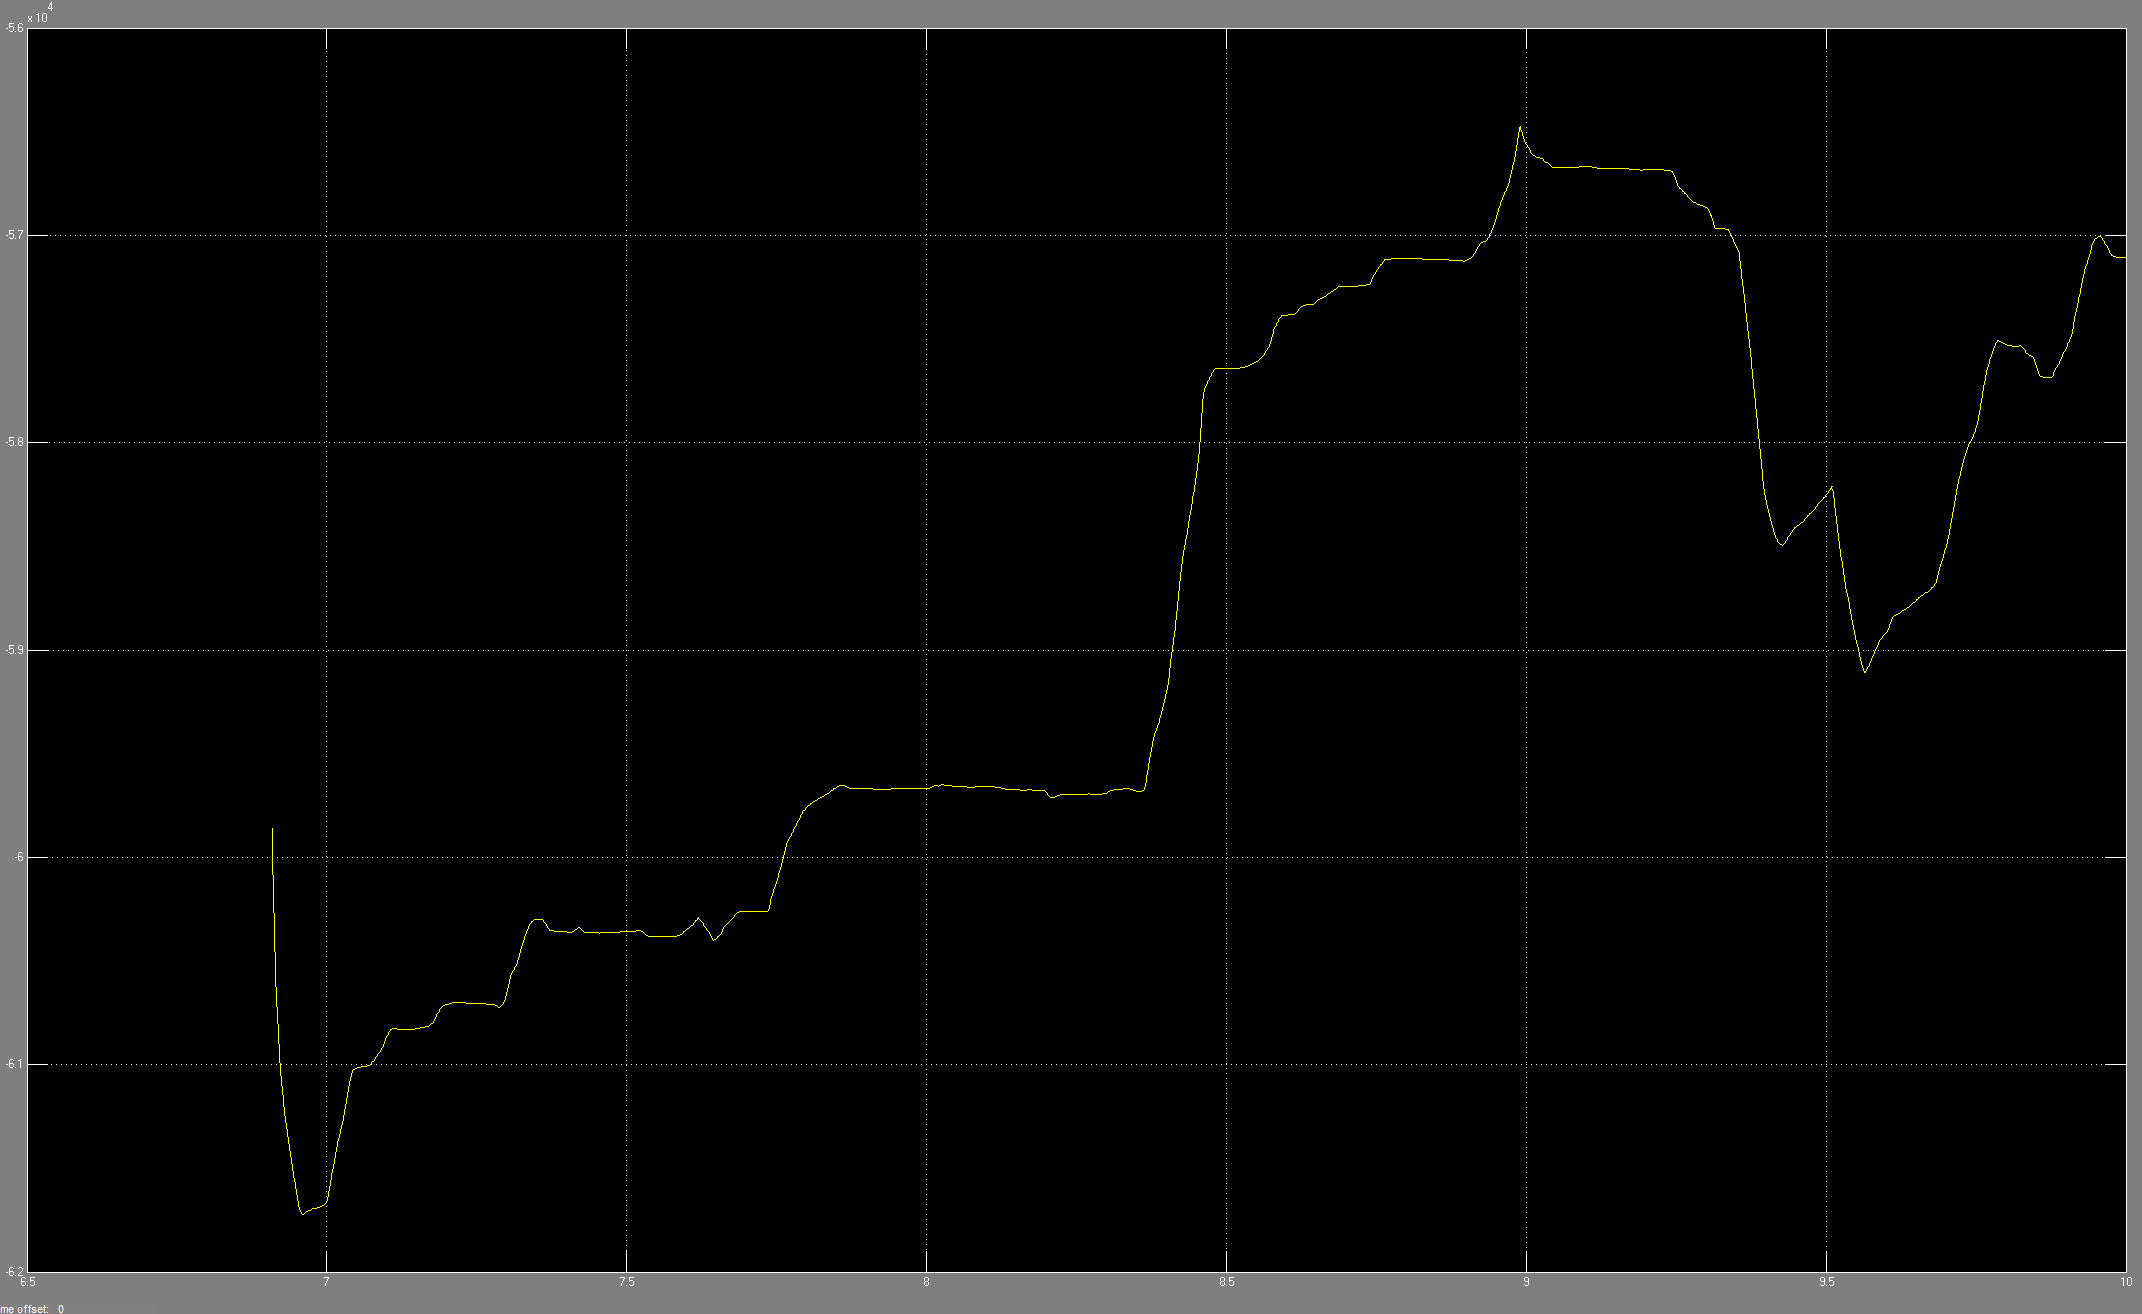
\includegraphics[scale=0.3]{q8_Theta2_step}\\
			\caption [WSpace]{Theta 2 for step torque}
		\end{centering}
	\end{figure}
	\subsection{}
	NA\newline
	\subsection{}
	NA\newline

	
